%-----------------------------------------------------------------------------%
\chapter{\babTiga}
%-----------------------------------------------------------------------------%
%\todo{tambahkan kata-kata pengantar bab 1 disini}
Penelitian ini bertujuan untuk mengevaluasi konfigurasi Hypervisor KVM yang disediakan secara langsung dalam konteks penggunaan \vm\ pada Apache Cloudstack. Tujuan utama adalah untuk memastikan bahwa \vm\ dapat mencapai kinerja yang optimal sesuai dengan spesifikasi sistem yang digunakan. Untuk mencapai tujuan ini, \saya akan melakukan penyesuaian konfigurasi atau tuning pada Hypervisor KVM dan kemudian membandingkannya dengan kondisi awal yang tidak mengalami tuning. Hasil pengujian akan dianalisis untuk menentukan apakah ada perbedaan signifikan dalam kinerja antara Hypervisor KVM yang telah dituning dengan yang belum dituning.

%-----------------------------------------------------------------------------%
\section{Tahapan Penelitian}
%-----------------------------------------------------------------------------%
\begin{figure}
    \centering
    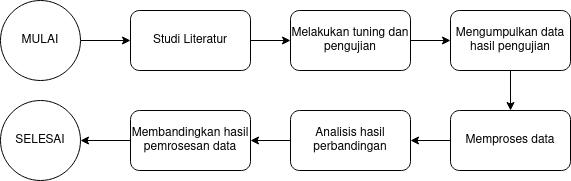
\includegraphics[width=1\textwidth]
    {assets/pics/tahapan-penelitian.png}
    \caption{Tahapan Penelitian}
    \label{fig:TahapanPenelitian}
\end{figure}

Penelitian ini akan dilakukan dalam beberapa tahap sesuai dengan diagram di gambar \ref{fig:TahapanPenelitian}. Tahap pertama melibatkan studi literatur untuk mengumpulkan semua informasi yang diperlukan untuk penelitian ini. Studi literatur ini penting karena memberikan dasar pengetahuan yang kuat tentang topik yang akan diteliti, memungkinkan \saya untuk memahami konteks dan kerangka kerja yang relevan.

Selanjutnya, penelitian melibatkan tuning terhadap Hypervisor KVM dan pengujian dilakukan dengan mengkompresi video menggunakan aplikasi Handbrake. Pengujian dengan Handbrake bertujuan untuk mengukur efisiensi dan kinerja Hypervisor KVM setelah tuning. Hasil pengujian Handbrake ini akan digunakan untuk membandingkan waktu kompresi video antara Hypervisor KVM yang tidak dituning dengan yang sudah dituning. Hasil dari perbandingan ini akan memberikan gambaran mengenai konfigurasi yang paling optimal dan sesuai, serta membantu dalam pemahaman lebih lanjut tentang pengaruh tuning terhadap performa Hypervisor KVM dalam konteks kompresi video.

%-----------------------------------------------------------------------------%
\section{Persiapan Lingkungan untuk Pengujian dan Analisis}
%-----------------------------------------------------------------------------%
\begin{figure}
    \centering
    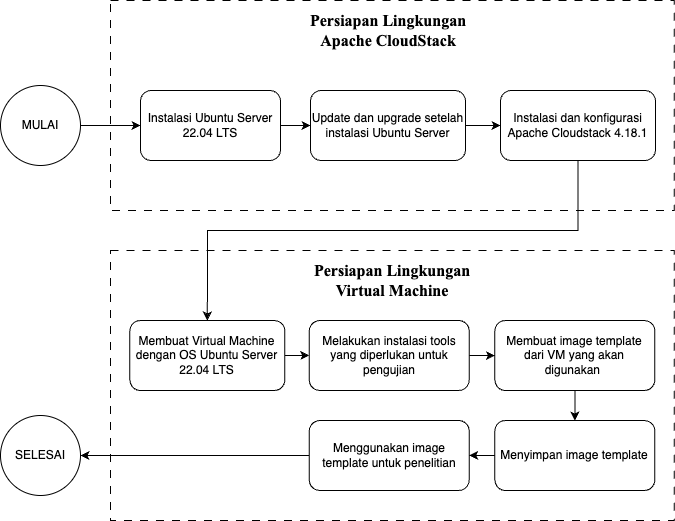
\includegraphics[width=1\textwidth]
    {assets/pics/persiapan_lingkungan_penelitian.png}
    \caption{Persiapan Lingkungan Penelitian}
    \label{fig:PersiapanLingkunganPenelitian}
\end{figure}


Proses persiapan lingkungan untuk pengujian dan analisis yang tergambar dalam gambar \ref{fig:PersiapanLingkunganPenelitian} menggambarkan serangkaian langkah sistematis yang penting untuk memastikan integritas hasil penelitian. Proses ini dimulai dengan tahap inisiasi yang meliputi instalasi Ubuntu Server 22.04 LTS, sebuah sistem operasi yang stabil dan sering digunakan untuk keperluan server. Instalasi ini menjadi landasan dasar bagi infrastruktur yang akan dikembangkan.

Setelah sistem operasi terinstal, dilakukan pembaruan dan peningkatan sistem operasi tersebut untuk memastikan semua komponen sistem berada pada versi terkini serta keamanan sistem terjaga. Langkah ini krusial untuk menutup potensi kerentanan yang mungkin ada pada sistem. Selanjutnya, Apache Cloudstack versi 4.18.1 diinstal dan dikonfigurasi. Apache Cloudstack berfungsi sebagai platform manajemen cloud yang memungkinkan pembuatan dan pengelolaan infrastruktur cloud yang kompleks, yang merupakan elemen kunci dalam penelitian ini.

Dalam pembuatan lingkungan virtual, dibuat \vm yang menggunakan sistem operasi yang sama, yaitu Ubuntu Server 22.04 LTS. Pembuatan VM ini memungkinkan simulasi berbagai skenario penelitian dalam lingkungan yang terisolasi. Selanjutnya, untuk keperluan analisis dan pengujian, Handbrake diinstal, dan video yang akan digunakan pun disiapkan.

Tahapan selanjutnya merupakan pembuatan image template dari VM yang telah dikonfigurasi. Proses ini memungkinkan duplikasi VM dengan cepat dan efisien untuk pengujian berulang atau skenario analisis yang berbeda, menjamin konsistensi lingkungan penelitian. Image template ini kemudian digunakan sebagai standar untuk penelitian lebih lanjut, memastikan bahwa setiap VM yang dibuat untuk tujuan pengujian memiliki konfigurasi yang identik.

Setelah semua dilakukan hal ini menandakan bahwa lingkungan penelitian telah siap untuk diuji dan dianalisis. Kesiapan lingkungan ini esensial untuk memastikan bahwa pengujian yang dilakukan dapat diulang dan hasilnya valid.

%-----------------------------------------------------------------------------%
\subsection{Instalasi dan Konfigurasi Apache Cloudstack}
%-----------------------------------------------------------------------------%
Dalam instalasi ini akan digunakan \f{Home Network} di IP 192.168.0.0/24. Pertama pastikan bahwa \f{tools} yang dibutuhkan sudah terinstall dengan perintah:

\begin{verbatim}
    sudo apt-get install -y openntpd openssh-server vim htop tar
    sudo apt-get install -y intel-microcode
\end{verbatim}

Perinyah ini akan menginstall \f{tools} openntpd, openssh-server, vim, htop, tar, dan intel-microcode. Setelah melakukan instalasi \f{tools} ini kemudian \saya\ akan mengganti password dari user root dengan perintah:

\begin{verbatim}
    sudo passwd root
\end{verbatim}

%-----------------------------------------------------------------------------%
\subsubsection{Pengaturan Jaringan}
%-----------------------------------------------------------------------------%
Melakukan pengaturan \f{Linux Bridge} yang akan menghandle jaringan CloudStack \f{public, guest, management} dan \f{storage}. Untuk penyederhanaan \saya\ akan menggunakan satu \f{bridge} yang bernama \textbf{cloudbr0} yang akan digunakan untuk semua jaringan ini. Untuk menginstall \f{tools} untuk melakukan \f{bridge} digunakan perintah:

\begin{verbatim}
    sudo apt-get install bridge-utils
\end{verbatim}

Setelah menginstall \f{tools} ini, \saya\ akan mengkonfigurasi \f{bridge} cloudbr0 dengan menggunakan netplan. Pertama pastikan bahwa seleuruh konfigurasi netplan sekarang di rename dengan menambahkan extensi .bak sebagai backup. Setelah itu buat file konfigruasi netplan dengan perintah:

\begin{verbatim}
    sudo nano /etc/netplan/01-netcfg.yaml
\end{verbatim}

Dengan perintah ini akan membuka text editor nano dengan file 01-netcfg.yaml. Isi file konfigurasi tersebut dengan:

\begin{listing}[H]
    \begin{minted}{yaml}
    network:
        version: 2
        renderer: networkd
        ethernets:
            enp2s0:
                dhcp4: false
                dhcp6: false
                optional: true
        bridges:
            cloudbr0:
                addresses: [192.168.0.10/24]
                routes:
                -   to: default
                    via: 192.168.0.1
                nameservers:
                    addresses: [1.1.1.1,8.8.8.8]
                interfaces: [enp2s0]
                dhcp4: false
                dhcp6: false
                parameters:
                    stp: false
                    forward-delay: 0
    \end{minted}
    \caption{Konfigurasi Netplan untuk Cloudbr0}
    \label{code:netplan_config}
\end{listing}

Dalam konfigurasi ini IP dari \f{bridge} cloudbr0 adalah 192.168.0.10/24 dan akan menggunakan DNS 1.1.1.1 dan 8.8.8.8. Setelah melakukan konfigurasi ini \saya\ akan mengaktifkan \f{bridge} cloudbr0 dengan perintah:

\begin{verbatim}
    sudo netplan generate
    sudo netplan apply
    sudo reboot
\end{verbatim}

Dengan perintah ini akan dilakukan netplan generate dan apply, setelah itu sistem melakukan reboot. Sampai sini pembuatan \f{bridge} cloudbr0 sudah selesai.

\subsubsection{Instalasi Cloudstack}
Pertama kita akan melakukan instalasi cloudstack-management dan juga mysql-server. Database yang akan digunakan adalah MySQL. Kita akan menggunakan perintah:

\begin{listing}[H]
    \begin{minted}{bash}
    sudo mkdir -p /etc/apt/keyrings
    wget -O- http://packages.shapeblue.com/release.asc | gpg --dearmor | sudo tee /etc/apt/keyrings/cloudstack.gpg > /dev/null

    echo deb [signed-by=/etc/apt/keyrings/cloudstack.gpg] http://packages.shapeblue.com/cloudstack/upstream/debian/4.18 / > /etc/apt/sources.list.d/cloudstack.list
    sudo apt-get update -y
    sudo apt-get install cloudstack-management mysql-server
    \end{minted}
\end{listing}

Perintah tersebut digunakan untuk menginstal CloudStack Management Server versi 4.18 dan MySQL Server dari repositori tertentu. Pertama, perintah membuat direktori untuk menyimpan kunci GPG yang digunakan untuk mengotentikasi paket dari repositori CloudStack. Kemudian, kunci GPG tersebut diunduh, didekompresi, dan disimpan dalam direktori yang telah dibuat. Selanjutnya, konfigurasi ditambahkan ke file sources.list.d untuk menandatangani paket-paket dari repositori CloudStack. Setelah itu, daftar paket diperbarui dan CloudStack Management Server serta MySQL Server diinstal menggunakan perintah apt-get. Selain ini juga akan dilakukan instalasi \f{tools} cloudstack usage dan billing yang bersifat opsional, dengan perintah:

\begin{verbatim}
    sudo apt-get install cloudstack-usage
\end{verbatim}

\subsubsection{Konfigurasi Database}
Setelah mysql server selesai di install akan dilakukan konfigurasi setting InnoDB di mysql server dengan perintah:

\begin{verbatim}
    sudo nano /etc/mysql/mysql.conf.d/mysqld.cnf
\end{verbatim}

Hapus semua isi file tersebut dan isi dengan:

\begin{listing}[H]
    \begin{minted}{ini}
    [mysqld]

    server_id = 1
    sql-mode="STRICT_TRANS_TABLES,NO_ENGINE_SUBSTITUTION,ERROR_FOR_DIVISION_BY_ZERO
    NO_ZERO_DATE,NO_ZERO_IN_DATE,NO_ENGINE_SUBSTITUTION"
    innodb_rollback_on_timeout=1
    innodb_lock_wait_timeout=600
    max_connections=1000
    log-bin=mysql-bin
    binlog-format = 'ROW'
    \end{minted}
    \caption{Konfigurasi mysqld.cnf}
    \label{code:mysql_config}
\end{listing}

Simpan konfigurasi dan setelah itu restart mysql server. Hal ini dilakukan agar mysql menggunakan setting yang terbaru. Untuk melakukan restart mysql server dapat dilakukan dengan perintah:

\begin{verbatim}
    systemctl restart mysql
\end{verbatim}

Setelah mysql server selesai di restart langkah selanjunya adalah deploy database untuk cloudstack. Deploy server ini harus dilakukan sebagai user root. Deploy dilakukan dengan perintah:

\begin{figure}
    \texttt{cloudstack-setup-databases cloud:cloud@localhost --deploy-as=root:password -i 192.168.0.10}
\end{figure}

IP yang digunakan adalah IP dari sistem host. Tunggu sampai deployment selesai, langkah ini akan selesai dalam beberapa menit.

\subsubsection{Konfigurasi Storage}
Pada tahap ini \saya\ akan melakukan konfigurasi untuk penyimpanan dari cloudstack. Pertama kita akan melakukan instalasi storage driver yang akan digunakan dengan perintah:

\begin{listing}[H]
    \begin{minted}{bash}
    sudo apt-get install nfs-kernel-server quota
    echo "/export  *(rw,async,no_root_squash,no_subtree_check)" > /etc/exports
    sudo mkdir -p /export/primary /export/secondary
    sudo exportfs -a
    \end{minted}
\end{listing}

Perintah \texttt{sudo apt-get install nfs-kernel-server quota} digunakan untuk menginstal perangkat lunak server NFS dan modul Quota pada sistem Linux. Selanjutnya, perintah \texttt{echo "/export *(rw,async,no\textunderscore root\textunderscore squash,no\textunderscore subtree\textunderscore check)" > /etc/exports} digunakan untuk menetapkan konfigurasi eksport NFS dengan opsi akses tertentu. Kemudian, perintah \texttt{sudo mkdir -p /export/primary /export/secondary} membuat direktori yang akan diakses oleh klien NFS. Terakhir, perintah \texttt{sudo exportfs -a} mengekspor semua direktori yang telah dikonfigurasi sebelumnya untuk diakses oleh klien NFS. Dengan demikian, rangkaian perintah ini mempersiapkan server NFS untuk berbagi data melalui jaringan. Setelah itu akan dilakukan konfigurasi NFS server dengan perintah:

\begin{listing}[H]
    \begin{minted}{bash}
    sed -i -e 's/^RPCMOUNTDOPTS="--manage-gids"$/RPCMOUNTDOPTS="-p 892 --manage-gids"/g' /etc/default/nfs-kernel-server
    sed -i -e 's/^STATDOPTS=$/STATDOPTS="--port 662 --outgoing-port 2020"/g' /etc/default/nfs-common
    echo "NEED_STATD=yes" >> /etc/default/nfs-common
    sed -i -e 's/^RPCRQUOTADOPTS=$/RPCRQUOTADOPTS="-p 875"/g' /etc/default/quota
    service nfs-kernel-server restart
    \end{minted}
\end{listing}

Perintah-perintah tersebut digunakan untuk mengubah konfigurasi pada server NFS dan Quota pada sistem Linux. Pertama, menggunakan \texttt{sed}, konfigurasi NFS Mount Daemon dan NFS Stat Daemon diubah untuk menggunakan port yang ditentukan dan mengaktifkan manajemen GID. Selanjutnya, layanan Stat Daemon diaktifkan dengan menambahkan opsi yang sesuai ke file konfigurasi NFS Common. Kemudian, konfigurasi RPC Quota Daemon diubah untuk menggunakan port yang ditentukan. Terakhir, layanan NFS Kernel Server di-restart untuk menerapkan perubahan konfigurasi yang telah dilakukan.

\subsubsection{Konfigurasi KVM}
Tahap selanjutnya adalah konfigurasi KVM dan cloudstack agent. Pertama install kvm dan cloudstack agent dengan perintah:

\begin{verbatim}
    sudo apt-get install qemu-kvm cloudstack-agent
\end{verbatim}

Setelah KVM dan cloudstack agent terinstall langkah selanjutnya adalah menjalankan perintah ini:

\begin{listing}[H]
    \begin{minted}{bash}
    sudo sed -i -e 's/\#vnc_listen.*$/vnc_listen = "0.0.0.0"/g' /etc/libvirt/qemu.conf
    sudo echo LIBVIRTD_ARGS=\"--listen\" >> /etc/default/libvirtd
    sudo systemctl mask libvirtd.socket libvirtd-ro.socket libvirtd-admin.socket libvirtd-tls.socket libvirtd-tcp.socket
    sudo systemctl restart libvirtd
    \end{minted}
\end{listing}

Perintah tersebut digunakan untuk mengkonfigurasi libvirt, sebuah toolkit untuk mengelola virtualisasi di Linux. Pertama, perintah \texttt{sed} digunakan untuk mengubah pengaturan dalam file konfigurasi \texttt{qemu.conf} agar libvirt dapat menerima koneksi VNC dari semua interface jaringan. Kemudian, argumen \texttt{--listen} ditambahkan ke konfigurasi libvirtd melalui file \texttt{/etc/default/libvirtd}, yang membuat libvirt mendengarkan koneksi dari interface jaringan. Selanjutnya, perintah \texttt{systemctl mask} digunakan untuk menonaktifkan unit-unit systemd yang terkait dengan libvirtd, seperti socket-soket yang tidak diperlukan, untuk menghindari aktivasi yang tidak diinginkan. Terakhir, layanan libvirtd di-restart agar perubahan konfigurasi dapat diterapkan.

Selanjutnya akan dilakukan konfigurasi default untuk libvirtd dengan perintah:

\begin{listing}[H]
    \begin{minted}{bash}
    echo 'listen_tls=0' >> /etc/libvirt/libvirtd.conf
    echo 'listen_tcp=1' >> /etc/libvirt/libvirtd.conf
    echo 'tcp_port = "16509"' >> /etc/libvirt/libvirtd.conf
    echo 'mdns_adv = 0' >> /etc/libvirt/libvirtd.conf
    echo 'auth_tcp = "none"' >> /etc/libvirt/libvirtd.conf
    systemctl restart libvirtd
    \end{minted}
\end{listing}

Perintah-perintah tersebut digunakan untuk mengkonfigurasi default pada file konfigurasi libvirt (libvirtd.conf). Pertama, dengan menambahkan \texttt{listen\_tls=0}, libvirt diminta untuk tidak mendengarkan koneksi TLS, sehingga mematikan mode tersebut. Kemudian, \texttt{listen\_tcp=1} mengaktifkan libvirt untuk mendengarkan koneksi TCP/IP. Penambahan \texttt{tcp\_port = "16509"} menetapkan port TCP yang akan digunakan oleh libvirt. Selanjutnya, dengan \texttt{mdns\_adv = 0}, mDNS advertise untuk penemuan otomatis layanan libvirt dimatikan. Terakhir, \texttt{auth\_tcp = "none"} mengatur libvirt untuk menerima koneksi TCP/IP tanpa melakukan otentikasi. Setelah perubahan-perubahan ini diterapkan, layanan libvirt di-restart agar konfigurasi baru dapat mulai berlaku. Penting untuk dicatat bahwa konfigurasi default ini hanya diperlukan saat setup awal, karena saat menambahkan host KVM dalam CloudStack, konfigurasi yang lebih aman menggunakan TLS akan diterapkan secara otomatis.

Pada host tertentu ditempat menjalankan docker dan service lainnya, dimungkinkan perlu untuk menambahkan konfigrasi berikut ini di \texttt{/etc/sysctl.conf} lalu jalankan \texttt{sysctl -p}

\begin{listing}[H]
    \begin{minted}{bash}
    nano /etc/sysctl.conf
    echo 'net.bridge.bridge-nf-call-arptables = 0' >> /etc/sysctl.conf
    echo 'net.bridge.bridge-nf-call-iptables = 0' >> /etc/sysctl.conf
    sysctl -p
    \end{minted}
\end{listing}

Pad perintah ini pertama, akan dibuka file \texttt{/etc/sysctl.conf} menggunakan editor teks nano. Kemudian, dengan menambahkan baris \texttt{net.bridge.bridge-nf-call-arptables = 0} dan \texttt{net.bridge.bridge-nf-call-iptables = 0} ke dalam file tersebut, Ini akan mematikan fungsi kernel yang biasanya dipanggil saat menggunakan Docker dan jembatan jaringan (bridge). Ini penting karena beberapa layanan, seperti Docker, kadang memerlukan konfigurasi khusus agar berjalan dengan lancar di lingkungan host yang kompleks. Terakhir, dengan menjalankan perintah \texttt{sysctl -p}, perubahan konfigurasi yang telah dibuat akan diterapkan tanpa harus me-reboot sistem, sehingga memungkinkan kernel untuk memuat ulang konfigurasi yang baru diterapkan.

Setelah itu kita akan mengenerate host id dengan uuid, hal ini dapat dilakukan dengan perintah:

\begin{listing}[H]
    \begin{minted}{bash}
    sudo apt-get install uuid
    UUID=$(uuid)
    echo host_uuid = \"$UUID\" >> /etc/libvirt/libvirtd.conf
    systemctl restart libvirtd
    \end{minted}
\end{listing}

Perintah ini digunakan untuk meng-generate UUID (Universally Unique Identifier) untuk host dan mengintegrasikannya ke dalam konfigurasi libvirtd. Perintah \texttt{UUID=\$(uuid)} digunakan untuk meng-generate UUID secara acak dan menyimpannya dalam variabel \texttt{UUID}. UUID adalah string panjang yang unik secara global dan digunakan untuk mengidentifikasi entitas secara unik di sistem. Kemudian, perintah \texttt{echo host\_uuid = \" \$UUID \"  >> /etc/libvirt/libvirtd.conf} menambahkan baris \texttt{host\_uuid = "<nilai UUID>"} ke dalam file konfigurasi \texttt{libvirtd.conf}. Fungsi baris ini adalah untuk menyimpan UUID host di konfigurasi libvirtd, yang akan digunakan oleh libvirt untuk mengidentifikasi host secara unik dalam lingkungan virtualisasi. Terakhir, perintah systemctl restart libvirtd digunakan untuk merestart layanan libvirtd agar perubahan konfigurasi yang telah dilakukan dapat diterapkan.

\subsubsection{Konfigurasi Firewall}
Untuk melakukan konfigruasi firewall kita dapat menggunakan perintah:

\begin{listing}[H]
    \begin{minted}{bash}
        # configure firewall rules to allow useful ports
        NETWORK=192.168.0.0/24
        iptables -A INPUT -s $NETWORK -m state --state NEW -p udp --dport 111 -j ACCEPT
        iptables -A INPUT -s $NETWORK -m state --state NEW -p tcp --dport 111 -j ACCEPT
        iptables -A INPUT -s $NETWORK -m state --state NEW -p tcp --dport 2049 -j ACCEPT
        iptables -A INPUT -s $NETWORK -m state --state NEW -p tcp --dport 32803 -j ACCEPT
        iptables -A INPUT -s $NETWORK -m state --state NEW -p udp --dport 32769 -j ACCEPT
        iptables -A INPUT -s $NETWORK -m state --state NEW -p tcp --dport 892 -j ACCEPT
        iptables -A INPUT -s $NETWORK -m state --state NEW -p tcp --dport 875 -j ACCEPT
        iptables -A INPUT -s $NETWORK -m state --state NEW -p tcp --dport 662 -j ACCEPT
        iptables -A INPUT -s $NETWORK -m state --state NEW -p tcp --dport 8250 -j ACCEPT
        iptables -A INPUT -s $NETWORK -m state --state NEW -p tcp --dport 8080 -j ACCEPT
        iptables -A INPUT -s $NETWORK -m state --state NEW -p tcp --dport 9090 -j ACCEPT
        iptables -A INPUT -s $NETWORK -m state --state NEW -p tcp --dport 16514 -j ACCEPT
        
        apt-get install iptables-persistent
    \end{minted}
\end{listing}

Perintah tersebut bertujuan untuk mengonfigurasi aturan firewall pada sistem menggunakan iptables, dengan fokus pada pembukaan port-port yang umum digunakan untuk layanan-layanan tertentu. Pertama, baris \texttt{NETWORK=192.168.0.0/24} mendefinisikan jaringan yang diizinkan melalui aturan firewall. Selanjutnya, setiap perintah \texttt{iptables -A INPUT ... -j ACCEPT} menambahkan aturan iptables untuk mengizinkan koneksi baru pada port tertentu dari jaringan yang telah ditentukan sebelumnya. Misalnya, perintah \texttt{iptables -A INPUT -s \$NETWORK -m state --state NEW -p udp --dport 111 -j ACCEPT} mengizinkan koneksi UDP baru pada port 111 dari jaringan yang telah ditentukan.

Aturan-aturan tersebut dirancang untuk membuka akses ke port-port yang umum digunakan oleh layanan-layanan seperti NFS, RPC, dan layanan manajemen tertentu. Setelah semua aturan ditambahkan, perintah \texttt{apt-get install iptables-persistent} digunakan untuk menginstal paket \texttt{iptables-persistent}, yang bertujuan agar konfigurasi aturan firewall yang telah dibuat akan dipertahankan dan diterapkan secara otomatis setiap kali sistem di-boot. Dengan demikian, langkah-langkah ini membantu menjaga keamanan sistem dengan memperbolehkan akses hanya ke port-port yang diperlukan dan memastikan bahwa aturan firewall tidak hilang setelah reboot.

Setelah itu kita harus menonaktifkan apparmor pada libvirtd, dikarenakan cloudstack melakukan berbagai macam hal yang mana bisa terblokir oleh mekanisme pertahanan seperti apparmor\cite{apacheHostInstallation}. Untuk mematikan apparmor dapat dilakukan dengan perintah:

\begin{listing}[H]
    \begin{minted}{bash}
    ln -s /etc/apparmor.d/usr.sbin.libvirtd /etc/apparmor.d/disable/
    ln -s /etc/apparmor.d/usr.lib.libvirt.virt-aa-helper /etc/apparmor.d/disable/
    apparmor_parser -R /etc/apparmor.d/usr.sbin.libvirtd
    apparmor_parser -R /etc/apparmor.d/usr.lib.libvirt.virt-aa-helper
    \end{minted}
\end{listing}

Perintah-perintah tersebut bertujuan untuk menonaktifkan AppArmor pada layanan libvirtd (Libvirt daemon). Langkah pertama adalah membuat symlink (tautan simbolis) dari file konfigurasi AppArmor yang berkaitan dengan libvirtd dan helpernya ke dalam direktori \texttt{/etc/apparmor.d/disable/}. Dengan melakukan ini, AppArmor diarahkan untuk mengabaikan atau menonaktifkan aturan-aturan yang telah didefinisikan untuk libvirtd. Selanjutnya, perintah \texttt{apparmor\_parser -R} digunakan untuk me-refresh aturan-aturan AppArmor yang terkait dengan libvirtd dan helpernya, sehingga aturan-aturan yang telah dinonaktifkan dengan symlink dapat diaplikasikan secara efektif.

Namun, penting untuk dicatat bahwa menonaktifkan AppArmor dapat meningkatkan risiko keamanan sistem karena menghilangkan lapisan proteksi yang diberikan oleh AppArmor terhadap layanan tersebut.


\subsubsection{Menjalankan CloudStack}
Sampai tahap ini instalasi cloudstack sudah selesai dan untuk menjalankan cloudstack dapat dengan menjalankan perintah ini:

\texttt{cloudstack-setup-management}

Setelah server manajemen sudah UP, cloudstack dapat diakses di http://192.168.0.10:8080 (IP dari cloudbr0) dan masuk dengan kredensial default yaitu admin/admin. Saat masuk pertama kali akan dilanjutkan dengan pengaturan Apache CloudStack. Dikonfigurasi ini dapat mengatur Zone, Network, Pod, Cluster, Host, Primary Storage, dan Secondary Storage. Pada setiap tahapnya dapat dikonfigurasikan dengan:

\begin{enumerate}
    \item Zone
    \begin{verbatim}
    Name - nama bebas
    Public DNS 1 - 8.8.8.8
    Public DNS 2 - 1.1.1.1
    Internal DNS1 - 192.168.0.1
    Hypervisor - KVM
    \end{verbatim}

    \item Network
    \begin{verbatim}
    Gateway - 192.168.0.1
    Netmask - 255.255.255.0
    VLAN/VNI - (kosong untuk vlan://untagged, 
                VXLAN untuk vxlan://untagged)
    Start IP - 192.168.0.20
    End IP - 192.168.0.50
    \end{verbatim}

    \item Pod
    \begin{verbatim}
    Name - nama bebas
    Gateway - 192.168.0.1
    Start/end reserved system IPs - 192.168.0.51 - 192.168.0.80
    \end{verbatim}

    \item Guest Traffic
    \begin{verbatim}
    VLAN/VNI range: 700-900
    \end{verbatim}

    \item Cluster
    \begin{verbatim}
    Name - nama bebas
    Hypervisor - pilih KVM
    \end{verbatim}

    \item Host
    \begin{verbatim}
    Hostname - 192.168.0.10
    Username - root
    Password - password user root
    \end{verbatim}

    \item Primary Storage
    \begin{verbatim}
    Name - nama bebas
    Scope - zone-wide
    Protocol - NFS
    Server - 192.168.0.10 [ubuntu server static IP]
    Path - /export/primary
    \end{verbatim}
    
    \item Secondary Storage
    \begin{verbatim}
    Provider - NFS
    Name - nama bebas
    Server - 192.168.100.10 [ubuntu server static ip]
    Path - /export/secondary
    \end{verbatim}
\end{enumerate}

Setelah konfigurasi selesai, pergi ke \texttt{Navigation>Infrasturcture>Summary} dan pastikan seluruh komponen sudah dinyalakan. Sekarang pengguna dapat menambahkan file iso yang diinginkan untuk membuat instance.

%-----------------------------------------------------------------------------%
\section{Tuning Hypervisor KVM}
%-----------------------------------------------------------------------------%
Tuning Hypervisor KVM yang dilakukan adalah dengan menambahkan flag instruksi yang tidak terdapat pada konfigurasi KVM default, dimana flag default dari KVM yang mendukung kompresi video hanyalah sse, dan sse2.

\begin{figure}
    \texttt{\textbf{fpu} vme \textbf{de pse tsc msr pae mce cx8 apic sep mtrr pge mca} \textbf{cmov pat pse36 clflush mmx fxsr sse sse2} ht \textbf{syscall nx} mmxext fxsr\textunderscore opt pdpe1gb rdtscp \textbf{lm} constant\textunderscore tsc \textbf{rep\textunderscore good} acc\textunderscore power\textbf{nopl} nonstop\textunderscore tsc \textbf{cpuid}  \textbf{extd\textunderscore apicid} aperfmperf \textbf{pni} pclmulqdq monitor ssse3 fma \textbf{cx16} sse4\textunderscore 1 sse4\textunderscore 2 movbe popcnt aes xsave avx f16c \textbf{lahf\textunderscore lm} cmp\textunderscore legacy \textbf{svm} extapic cr8\textunderscore legacy abm sse4a misalignsse\textbf{3dnowprefetch} osvw ibs xop skinit wdt lwp fma4 tce nodeid\textunderscore msr tbmtopoext perfctr\textunderscore core perfctr\textunderscore nb bpext ptsc mwaitx cpb hw\textunderscore pstate ssbd \textbf{vmmcall} fsgsbase bmi1 avx2 smep bmi2 xsaveopt arat npt lbrv svm\textunderscore locknrip\textunderscore save tsc\textunderscore scale vmcb\textunderscore clean flushbyasid decodeassists pausefilter pfthreshold avic v\textunderscore vmsave\textunderscore vmload vgif overflow\textunderscore recov}
    \caption{Seluruh flag instruksi di Host}
    \label{fig:flag_kvm_host}
\end{figure}

Terlihat pada gambar \ref{fig:flag_kvm_host} adalah keseluruhan flag instruksi dari sistem host, sedangkan text yang ditajamkan adalah flag instruksi bawaan default dari hypervisor KVM. Dari sini flag yang berguna untuk melakukan kompresi video dan ditajamkan hanyalah sse dan sse2, hal ini menandakan bahwa KVM tidak mengaktifkan keseluruhan flag instruksi meskipun pada sistem host sudah mendukung flag instruksinya. Beberapa flag yang berguna untuk melakukan kompresi video dan tidak dinyalakan oleh hypervisor KVM adalah SSE3, SSE4\_1, dan SSE4\_2. 

\saya\ dapat mengaktifkan flag tersebut untuk digunakan oleh \vm\ yang menggunakan hypervisor KVM. Untuk melakukan tuning \saya\ dapat menggunakan tools virsh untuk mengubah konfigurasi \vm dari CloudStack. Secara default konfigurasi dari \vm di CloudStack akan seperti ini:

\begin{listing}[H]
    \begin{minted}{xml}
        <domain type='kvm'>
        
            ...
            
            <cpu mode='custom' match='exact' check='full'>
                <model fallback='forbid'>qemu64</model>
                <feature policy='require' name='x2apic'/>
                <feature policy='require' name='hypervisor'/>
                <feature policy='require' name='lahf_lm'/>
            </cpu>
            
            ...
            
        </domain>
    \end{minted}
    \caption{Konfigurasi default dari KVM}
    \label{code:default_kvm_xml}
\end{listing}

Terlihat dari kode \ref{code:default_kvm_xml} bahwa feature yang dinyalakan tidak memuat sse3, sse4\_1, dan sse4\_2. Untuk itu \saya\ dapat menambahkan fitur tersebut sehingga \vm dapat menggunakan flag instruksi tersebut. Perubahahan yang akan \saya lakukan akan seperti ini:

\begin{listing}[H]
    \begin{minted}{xml}
        <domain type='kvm'>
        
            ...
            
            <cpu mode='custom' match='exact' check='full'>
                <model fallback='forbid'>qemu64</model>
                <feature policy='require' name='x2apic'/>
                <feature policy='require' name='hypervisor'/>
                <feature policy='require' name='lahf_lm'/>
                <feature policy='require' name='sse3'/>
                <feature policy='require' name='sse4_1'/>
                <feature policy='require' name='sse4_2'/>
            </cpu>
            
            ...
            
        </domain>
    \end{minted}
    \caption{Konfigurasi tuning KVM}
    \label{code:tuned_kvm_xml}
\end{listing}

Jika sudah dilakukan penambahan fitur seperti di kode \ref{code:tuned_kvm_xml} sekarang \vm yang menggunakan Hypervisor KVM sudah bisa mendukung set instruksi tersebut.

%-----------------------------------------------------------------------------%
\section{Pengujian Kompresi Video Dengan HandBrake}
%-----------------------------------------------------------------------------%
Untuk menguji dan membandingkan kinerja Hypervisor KVM sebelum dan sesudah tuning, {\saya} akan menggunakan software HandBrake, sebuah software kompresi video yang sudah banyak digunakan. Proses ini melibatkan penggunaan HandBrake untuk kompresi video pada dua lingkungan \vm\ yang berbeda, yang mana satu menggunakan KVM yang belum di-tuning dan yang lainnya menggunakan KVM yang telah di-tuning. Tujuan dari pengujian ini adalah untuk mengevaluasi sejauh mana tuning Hypervisor KVM dapat mempengaruhi kecepatan kompresi video.

HandBrake dipilih karena kemampuannya yang baik dalam mengkompresi video dan mudah untuk digunakan\cite{Folgar2014eg}. Dalam pengujian ini, video yang akan digunakan adalah "COSTA RICA IN 4K 60fps HDR (ULTRA HD)" yang diunduh dari YouTube dengan resolusi video yang digunakan adalah 2K. Video ini dipilih karena resolusi tingginya, yang memberikan tantangan yang baik untuk menguji efisiensi kompresi video pada kedua lingkungan \vm. 

Parameter penting yang akan diukur dalam pengujian ini adalah: 

\begin{enumerate}
    \item \textbf{\f{Time Elapsed}}
    
    \f{Time Elapsed} atau berapa lama waktu yang dibutuhkan oleh masing-masing \vm\ untuk menyelesaikan proses kompresi video.
        
    \item \textbf{\f{Structural Similarity Index Measure Score}}
    
    Structural Similarity Index Measure adalah cara untuk menilai kesamaan dari 2 buah gambar, untuk melihat apakah terjadi penurunan kualitas atau perbedaan yang besar antara gambar yang belum di compress dengan gambar yang sudah di compress.
\end{enumerate}


Data ini yang akan memberikan gambaran yang jelas mengenai perbedaan kinerja antara KVM yang telah di-tuning dengan yang belum.

Spesifikasi dari \vm\ yang akan digunakan dalam pengujian ini adalah sebagai berikut:
\begin{itemize}
    \item \textbf{Cloud Platform}: Apache CloudStack 4.18.1
    \item \textbf{OS}: Ubuntu Server 22.04 LTS
    \item \textbf{CPU}: 1 CPU x 1.00 Ghz
    \item \textbf{Memory}: 1024 MB
\end{itemize} 

Perintah yang digunakan untuk melakukan kompresi video dengan handbrake adalah sebagai berikut:

\begin{verbatim}
    ./HandBrakeCLI -i /path/to/input.mov -o /path/to/output.mp4
    -e x264 -q 28 -r 15 -B 64 -X 1280 -O
\end{verbatim}

Dengan perintah ini \saya akan melakukan kompresi video dengan codec x264. Codec yang dikembangkan oleh VideoLAN yang sudah banyak digunakan dikarenakan mampu untuk melakukan kompresi video yang baik dan rendahnya tingkat penurunan kualitas gambar.

%-----------------------------------------------------------------------------%
\section{Analisis Pengujian}
%-----------------------------------------------------------------------------%
Dalam analisis ini, waktu kompresi untuk Hypervisor KVM yang belum di-tuning akan disebut sebagai $T_{\mathrm{default}}$, sementara waktu kompresi untuk Hypervisor KVM yang telah di-tuning akan disebut sebagai $T_{\mathrm{tuned}}$. Waktu kompresi ini akan diambil dari logs HandBrake yang telah melakukan kompresi video. Untuk mengetahui apakah terdapat perbedaan yang signifikan, \saya\ dapat menggunakan formula speedup. 

\[ \mathrm{Speedup} = \frac{T_{\mathrm{default}}}{T_{\mathrm{tuned}}} \]

Jika nilai speedup lebih dari 1, ini menandakan bahwa proses kompresi dengan Hypervisor KVM yang sudah di-tuning lebih cepat dibandingkan dengan yang belum di-tuning. 

Pengujian akan dilakukan sebanyak kurang lebih sepuluh kali dan nantinya akan ditampilkan dalam bentuk grafik. Akan terdapat grafik \f{line chart} dengan dua garis dimana masing-merepresentasikan $T_{\mathrm{default}}$ dan $T_{\mathrm{tuned}}$.

Selain menganalisis waktu kompresi video, \saya\ juga akan melakukan analisis untuk menilai kualitas video yang telah dikompresi. Analisis ini akan melibatkan perbandingan nilai dari \f{Structural Similarity Index Measure} (SSIM) antara video yang dikompres menggunakan Hypervisor KVM default dan Hypervisor KVM yang telah di-tuning. SSIM adalah metrik yang mengukur kesamaan visual antara dua video. Semakin tinggi nilai SSIM, semakin mirip video yang dikompres dengan versi aslinya. Oleh karena itu, nilai SSIM yang lebih tinggi menunjukkan kualitas kompresi yang lebih baik, dimana integritas visual dari video asli lebih terjaga.


\iffalse
Selanjutnya, \saya\ akan menghitung efisiensi dari tuning Hypervisor KVM ini. Untuk mengetahui efisiensi, \saya\ dapat menggunakan formula efisiensi.

\[ \mathrm{Efficiency} = \frac{\mathrm{Speedup}}{\frac{R_{\mathrm{tuned}}}{R_{\mathrm{default}}}} \]


Tujuan menghitung efisiensi ini adalah untuk mengetahui seberapa efektif tuning dilakukan dalam menggunakan sumber daya yang ada, seperti penggunaan CPU dan memori. Perhitungan ini penting untuk menilai kinerja tuning dalam konteks keseluruhan penggunaan sumber daya, tidak hanya kecepatan kompresi.
\fi

% Time Measurement
%$T_{\mathrm{default}}$, $T_{\mathrm{tuned}}$
%\[ T_{\mathrm{default}}, \quad T_{\mathrm{tuned}} \]

% Speedup
%$\mathrm{Speedup} = \frac{T_{\mathrm{default}}}{T_{\mathrm{tuned}}}$
%\[ \mathrm{Speedup} = \frac{T_{\mathrm{default}}}{T_{\mathrm{tuned}}} \]



\iffalse
%-----------------------------------------------------------------------------%
\section{Satu Persamaan}
%-----------------------------------------------------------------------------%

\noindent \begin{align}\label{eq:garis}
    \cfrac{y - y_{1}}{y_{2} - y_{1}} = 
    \cfrac{x - x_{1}}{x_{2} - x_{1}}
\end{align}

\equ~\ref{eq:garis} diatas adalah persamaan garis. 
\equ~\ref{eq:garis} dan \ref{eq:bola} sama-sama dibuat dengan perintah \bslash
align. 
Perintah ini juga dapat digunakan untuk menulis lebih dari satu persamaan. 

\noindent \begin{align}\label{eq:bola}
    \underbrace{|\overline{ab}|}_{\text{pada bola $|\overline{ab}| = r$}} 
    = \sqrt[2]{(x_{b} - x_{a})^{2} + (y_{b} - y_{a})^{2} + 
        \vert\vert(z_{b} - z_{a})^{2}}
\end{align}

%-----------------------------------------------------------------------------%
\section{Lebih dari Satu Persamaan}
\label{sec:multiEqu}
%-----------------------------------------------------------------------------%
\noindent \begin{align}\label{eq:matriks}	
    |\overline{a} * \overline{b}| &= |\overline{a}| |\overline{b}| \sin\theta 
    \\[0.2cm]
    \overline{a} * \overline{b} &=  
    \begin{array}{| c c c |}
        \hat{i} & x_{1} & x_{2} \\
        \hat{j} & y_{1} & y_{2} \\
        \hat{k} & z_{1} & z_{2} \\
    \end{array} \nonumber \\[0.2cm]
    &= \hat{i} \,
    \begin{array}{ | c c | }
        y_{1} & y_{2} \\
        z_{1} & z_{2} \\
    \end{array} 
    + \hat{j} \,
    \begin{array}{ | c c | }
        z_{1} & z_{2} \\
        x_{1} & x_{2} \\
    \end{array} 
    + \hat{k} \,	
    \begin{array}{ | c c | }
        x_{1} & x_{2} \\
        y_{1} & y_{2} \\
    \end{array}
    \nonumber
\end{align}

Pada \equ~\ref{eq:matriks} dapat dilihat beberapa baris menjadi satu bagian 
dari \equ~\ref{eq:matriks}. 
Sedangkan dibawah ini dapat dilihat bahwa dengan cara yang sama, \equ~
\ref{eq:gabungan1}, \ref{eq:gabungan2}, dan \ref{eq:gabungan3} memiliki nomor 
persamaannya masing-masing. 

\noindent \begin{align}\label{eq:gabungan1}	
    \int_{a}^{b} f(x)\, dx + \int_{b}^{c} f(x) \, dx = \int_{a}^{c} f(x) \, dx
    \\\label{eq:gabungan2}
    \lim_{x \to \infty} \frac{f(x)}{g(x)} = 0 \hspace{1cm} 
    \text{jika pangkat $f(x)$ $<$ pangkat $g(x)$} \\\label{eq:gabungan3}
    a^{m^{a \, ^{n}\log b }} = b^{\frac{m}{n}}
\end{align}
\fi
